% !TEX root = ../Monografia.tex
\chapter{Extração de Relações e Construção do Grafo}
\label{cap:extracao}

Este capítulo descreve a parte azul da Figura~\ref{fig:pipeline}: como cada artigo foi transformado em
relações estruturadas por um LLM, como essas relações foram filtradas e ligadas aos \emph{tickers} das
empresas, e como formam o grafo dinâmico usado nos testes. O capítulo termina com a validação da
extração e com uma descrição do grafo resultante.

%--------------------------------------------------------------------
\section{Formulação da tarefa}
\label{sec:tarefa}

Para cada artigo, o modelo recebe o título, a data, os \emph{tickers} marcados no corpus e o texto,
truncado em 8.000 caracteres, e devolve uma lista de tuplas
\begin{equation}
  (\text{agent\_a},\ \text{agent\_b},\ \text{relation\_type},\ \text{direction},\ \text{strength}),
  \label{eq:tupla}
\end{equation}
às quais se acrescenta a data de publicação do artigo. Cada tupla descreve uma ação de um agente
econômico sobre outro: \texttt{agent\_a} é quem age, \texttt{agent\_b} é quem recebe o efeito,
\texttt{relation\_type} é a ação, numa expressão verbal curta e livre (``investe em'', ``fornece para'',
``concorre com'', ``eleva juros sobre''), \texttt{direction} é o efeito sobre \texttt{agent\_b}, positivo
ou negativo, e \texttt{strength} é a força e a certeza do efeito, entre 0 e 1.

O prompt (Apêndice~\ref{ap:prompt}) define o que é um agente econômico: empresas, índices, bancos
centrais, governos e reguladores, moedas e criptoativos, \emph{commodities}, setores, instituições e
fundos, e pessoas economicamente relevantes. Define também o que não é: métricas contábeis, como
receita, lucro ou dividendos; grupos genéricos, como ``investidores'' ou ``analistas''; e o próprio
veículo que publica a notícia. As regras principais são:
\begin{itemize}
  \item os dois agentes precisam estar nomeados no artigo, e nenhuma relação pode ser inferida de
        conhecimento externo;
  \item a direção é o efeito sobre \texttt{agent\_b}; um efeito mútuo gera duas tuplas;
  \item a força segue faixas: 0,8 a 1,0 para efeitos explícitos e materiais, 0,4 a 0,7 para efeitos
        declarados mas modestos ou indiretos, 0,1 a 0,3 para efeitos especulativos;
  \item no máximo oito tuplas por artigo, e uma lista vazia é uma resposta válida.
\end{itemize}

O formato da resposta é imposto por decodificação restrita: o servidor de inferência recebe um esquema
JSON que fixa os cinco campos, os valores possíveis da direção, o intervalo da força e o máximo de oito
itens, e só permite ao modelo gerar sequências que obedeçam a ele. Toda resposta é, assim, um JSON
válido. A força ainda é limitada a $[0,1]$ na gravação, porque o esquema garante o tipo numérico, mas
nem sempre a faixa.

O limite de 8.000 caracteres preserva 83,9\% de todo o texto e trunca apenas 5,1\% das unidades,
medidos nas 401.609 unidades da amostra de 25\%, cuja mediana tem 2.999 caracteres. O tamanho do contexto do
modelo é calculado pelo pior caso de caracteres por \emph{token}, para que nenhum artigo seja cortado em
silêncio.

%--------------------------------------------------------------------
\section{Modelo e execução}
\label{sec:modelo-llm}

A extração usa um modelo de pesos abertos executado localmente, o que dá custo previsível, versão fixa e
reprodutibilidade. Dois modelos de 14 bilhões de parâmetros foram comparados nos mesmos 200 artigos, com
o mesmo prompt: o Qwen2.5-14B-Instruct \citep{qwen2024}, um modelo de instrução, e o DeepSeek-R1-14B, um
modelo destilado de raciocínio. Numa conferência manual de 40 tuplas de cada um, cerca de dois terços das
tuplas do Qwen2.5 eram relações válidas entre agentes, contra cerca de um quarto das do DeepSeek-R1, que
preenchia a lista até o limite de oito tuplas em 30\% dos artigos (5\% no Qwen2.5) e usava métricas
contábeis e grupos genéricos como agentes com o dobro da frequência. O Qwen2.5 deixa vazios cerca de 40\%
dos artigos, na maioria avisos de ex-dividendo, listas de cotações e textos padronizados, e foi 39\% mais
rápido. Uma versão de 7 bilhões de parâmetros foi descartada num teste anterior por inventar relações.

A extração rodou em GPUs alugadas por hora, com o servidor de inferência Ollama, a cerca de um artigo por
segundo. Cada resposta é gravada imediatamente em disco, e cada tupla carrega uma versão calculada como
\emph{hash} do prompt, do esquema, do limite de caracteres e do nome do modelo, de modo que resultados de
configurações diferentes nunca se misturam. Foram processadas 572.762 unidades, sem nenhuma falha, que
produziram 1.270.582 tuplas; 327.406 unidades (57\%) tiveram ao menos uma relação, com média de 3,9 tuplas
cada.

%--------------------------------------------------------------------
\section{Filtro de ruído}
\label{sec:ruido}

Apesar das instruções, parte das tuplas não descreve uma relação entre dois agentes econômicos. Um
filtro baseado em regras e listas \emph{marca} cada tupla com o motivo de ruído, sem apagá-la: um dos
lados é um grupo genérico, como ``investidores'' (7,3\% das tuplas); a relação é uma comparação de
desempenho (2,2\%) ou o pertencimento a um índice (1,5\%); o agente é o veículo ou a casa de análise que
publica (1,1\%); os dois lados são o mesmo agente (0,8\%); um dos lados é uma métrica contábil (0,8\%); ou a
relação é de organograma, como a nomeação de um dirigente (0,2\%). Restam 1.093.431 tuplas limpas, 86,1\%
do total. Indicadores macroeconômicos e setores não são tratados como ruído (``Fed $\to$ bancos''),
porque são exatamente as entidades não negociadas que o trabalho quer capturar. A qualidade das tuplas
limpas é medida na Seção~\ref{sec:anotacao}.

%--------------------------------------------------------------------
\section{Ligação de entidades a tickers}
\label{sec:link}

Para cruzar o grafo com os preços, cada nome de agente precisa ser associado, quando for o caso, ao
\emph{ticker} da empresa. A ligação é feita em quatro passos:
\begin{enumerate}
  \item \textbf{Candidatos.} Para cada nome distinto, um procedimento determinístico monta uma lista
        fechada de \emph{tickers} candidatos, em ordem de força da evidência: o \emph{ticker} escrito no
        próprio nome (``NASDAQ: AAPL''); o nome igual ao da listagem oficial da Nasdaq; o nome que já é
        um \emph{ticker} (``AMD''); os \emph{tickers} marcados nos artigos em que o nome aparece; e nomes
        parecidos na listagem. O universo de \emph{tickers} é a união dos que têm preço no FNSPID e dos
        marcados no corpus.
  \item \textbf{Escolha pelo LLM.} Um modelo menor, o Qwen2.5-7B-Instruct, recebe o nome, o contexto e os
        candidatos e só pode \emph{escolher} um deles ou ``nenhum'', porque os candidatos entram no
        esquema como uma enumeração fechada. O modelo também classifica o tipo do agente (empresa,
        fundo, banco central, país, \emph{commodity} etc.).
  \item \textbf{Regras.} Só empresas e fundos recebem \emph{ticker}, e o \emph{ticker} escolhido precisa
        ter nome compatível com o agente ou evidência forte no texto. Um \emph{ticker} entre parênteses
        no nome é tratado só como evidência: ``petróleo (WTI)'' não é a empresa W\&T Offshore, cujo
        \emph{ticker} é WTI.
  \item \textbf{Verificação.} Um segundo passo, com uma pergunta de sim ou não ao modelo, derruba
        colisões com \emph{tickers} de empresas estrangeiras ou homônimas, exceto controladoras e fundos
        de índice.
\end{enumerate}

Foram ligados 304.430 nomes distintos. Entre as tuplas limpas, 52,3\% têm \emph{ticker} em ao menos um
dos lados e 13,2\% nos dois. Por falta de orçamento, a verificação do passo 4 não foi aplicada a 434
\emph{tickers} que surgiram na ampliação da amostra (875 menções), dos quais se estima que cerca de um
quarto esteja errado.

%--------------------------------------------------------------------
\section{O grafo dinâmico}
\label{sec:grafo}

\subsection{Nós}

Cada nó do grafo é um agente. Para empresas com \emph{ticker}, o nó é o \emph{ticker}; para os demais,
um identificador canônico do nome. A construção dos nós segue regras que corrigem os erros mais comuns
da unificação de nomes:
\begin{itemize}
  \item o nome canônico sugerido pelo LLM só é aceito se for compatível com o nome original (mesmo
        \emph{token}, prefixo ou sigla), o que evita fusões erradas, como um banco central estrangeiro
        unido ao Federal Reserve;
  \item prefixos de país são removidos quando a versão sem prefixo existe com o mesmo tipo (``US
        Federal Reserve'' e ``Federal Reserve''), exceto para empresas;
  \item classes de ação da mesma empresa são unidas (GOOG e GOOGL);
  \item nomes que coincidem com \emph{tickers} de outras coisas recebem o tipo no identificador (o milho,
        \emph{corn}, não é o fundo de \emph{ticker} CORN);
  \item uma lista manual resolve os casos restantes, como FOMC e Federal Reserve, ou WTI, Brent e
        petróleo.
\end{itemize}

O resultado tem 255.384 nós, dos quais 5.979 têm \emph{ticker}. O nó do Federal Reserve, por exemplo,
reúne 200 grafias diferentes. A Tabela~\ref{tab:nos} mostra os nós com mais eventos, que já indicam o
papel das entidades não negociadas no grafo.

\begin{table}[htbp]
\centering
\small
\caption{Nós com mais eventos no grafo.}
\label{tab:nos}
\begin{tabular}{llr@{\hspace{1.2em}}llr}
\toprule
nó & tipo & eventos & nó & tipo & eventos \\
\midrule
Federal Reserve & banco central & 30.769 & Google & empresa & 7.945 \\
petróleo & \emph{commodity} & 19.285 & JPMorgan Chase & empresa & 7.144 \\
China & país & 15.726 & Goldman Sachs & empresa & 7.109 \\
Apple & empresa & 12.779 & Microsoft & empresa & 6.844 \\
S\&P 500 & índice & 12.584 & economia dos EUA & macro & 6.005 \\
Amazon & empresa & 9.231 & governo dos EUA & governo & 5.975 \\
Banco Central Europeu & banco central & 8.543 & ouro & \emph{commodity} & 5.931 \\
dólar & moeda & 8.052 & & & \\
\bottomrule
\end{tabular}
\end{table}

\subsection{Eventos e classes de relação}

Cada tupla limpa vira um evento datado entre dois nós, com peso $w=\pm\,\text{força}$, conforme a
direção. O campo \texttt{relation\_type} é livre, e o modelo produziu 184.035 expressões distintas.
Elas foram agrupadas em 16 classes por expressões regulares, e a expressão original é mantida no
evento. A Tabela~\ref{tab:classes} mostra as classes, sua frequência e o sinal médio. As tuplas em que a
unificação dos nomes produziu um laço (uma empresa e as próprias ações, por exemplo) não viram arestas.

\begin{table}[htbp]
\centering
\small
\caption{Classes de relação: participação nos eventos e sinal médio ($+1$ positivo, $-1$ negativo).}
\label{tab:classes}
\begin{tabular}{lrr@{\hspace{2.5em}}lrr}
\toprule
classe & eventos & sinal & classe & eventos & sinal \\
\midrule
impacto & 32,1\% & $+0{,}01$ & analista & 3,1\% & $+0{,}25$ \\
outras & 14,0\% & $+0{,}08$ & negócios & 2,9\% & $+0{,}71$ \\
concorrência & 9,2\% & $-0{,}87$ & financiamento & 2,3\% & $+0{,}26$ \\
participação & 7,3\% & $+0{,}43$ & monetária & 2,0\% & $-0{,}23$ \\
fusões e aquisições & 7,0\% & $+0{,}41$ & governança & 0,9\% & $+0{,}63$ \\
cadeia de suprimentos & 6,1\% & $+0{,}22$ & política comercial & 0,9\% & $-0{,}02$ \\
parceria & 4,4\% & $+0{,}79$ & retorno de capital & 0,3\% & $-0{,}26$ \\
legal e regulatória & 4,1\% & $-0{,}48$ & posicionamento & 3,3\% & $-0{,}19$ \\
\bottomrule
\end{tabular}
\end{table}

O sinal médio mostra que as classes têm leituras econômicas coerentes: parcerias e negócios são quase
sempre positivos, processos e regulação tendem a ser negativos, e a concorrência é quase sempre
negativa ($-0{,}87$), porque o ganho de uma empresa é descrito como perda da rival. Essa última
característica será importante na interpretação dos resultados (Capítulo~\ref{cap:res-correlacao}).

\subsection{O grafo numa data}

O grafo final tem 1.064.801 eventos limpos, entre 673.261 pares de nós distintos. Ele não é
materializado para cada data: o grafo em $t$ é obtido agregando os eventos da janela anterior a $t$
com o peso da Equação~\eqref{eq:peso-evento}, o que leva cerca de 40 milissegundos por data. Como os
eventos com data igual ou posterior a $t$ nunca entram, o grafo pode ser consultado em qualquer data sem
informação futura.

A Figura~\ref{fig:grafo-exemplo} mostra um recorte real do grafo. Os três grandes bancos aparecem ligados
ao Federal Reserve, as petroleiras ao petróleo, e Apple e Boeing à China, com efeito negativo no ano da
disputa comercial. As arestas diretas entre os bancos são negativas, de concorrência. É dessa estrutura
que saem os atributos de par da Seção~\ref{sec:atributos}: JPMorgan e Bank of America têm exposição
comum positiva (0,18 nessa data), porque se ligam à mesma entidade com o mesmo sinal, e a exposição comum
entre um banco e uma petroleira é praticamente nula.

\begin{figure}[htbp]
\centering
% Subgrafo real: eventos dos 365 dias anteriores a 2019-01-02, meia-vida de 90 dias.
% Pesos = soma dos eventos com sinal e decaimento (Equação peso-evento).
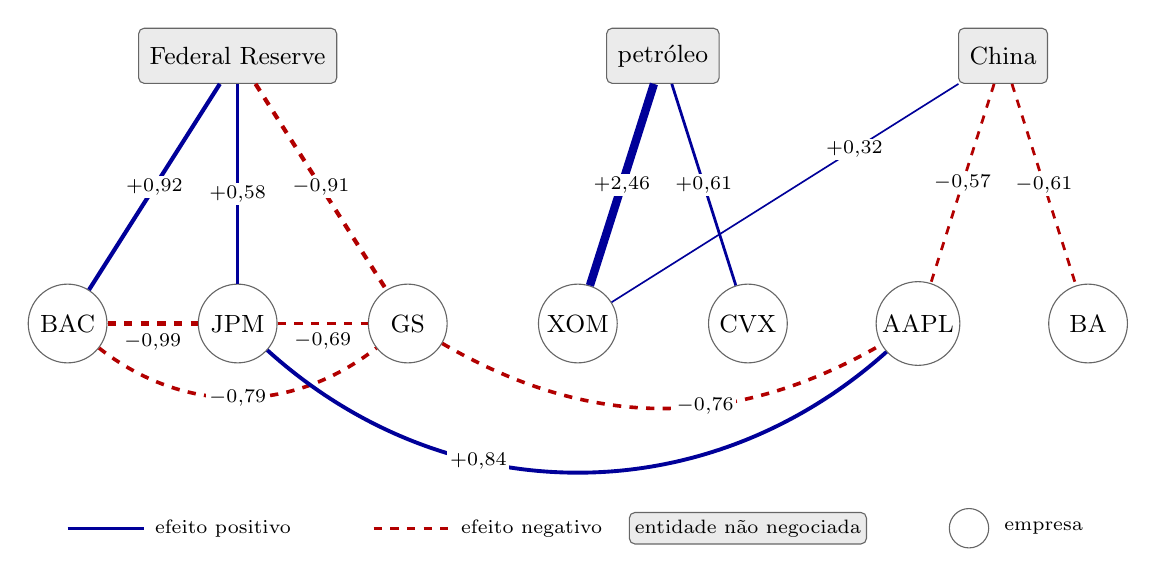
\begin{tikzpicture}[
  x=1.08cm, y=1cm,
  ent/.style={draw=black!60, fill=black!8, rounded corners=2pt, font=\small, inner sep=4pt, minimum height=7mm},
  emp/.style={draw=black!60, fill=white, circle, font=\small, inner sep=1.5pt, minimum size=10mm},
  efpos/.style={draw=blue!60!black},
  efneg/.style={draw=red!70!black, dashed},
  rot/.style={font=\scriptsize, fill=white, inner sep=1pt},
]
% entidades não negociadas
\node[ent] (fed)   at (2,3.4)  {Federal Reserve};
\node[ent] (oil)   at (7,3.4)  {petróleo};
\node[ent] (china) at (11,3.4) {China};
% empresas
\node[emp] (bac)  at (0,0)  {BAC};
\node[emp] (jpm)  at (2,0)  {JPM};
\node[emp] (gs)   at (4,0)  {GS};
\node[emp] (xom)  at (6,0)  {XOM};
\node[emp] (cvx)  at (8,0)  {CVX};
\node[emp] (aapl) at (10,0) {AAPL};
\node[emp] (ba)   at (12,0) {BA};
% exposição a entidades (espessura proporcional ao módulo)
\draw[efpos, line width=1.5pt] (fed) -- node[rot, pos=0.5] {$+0{,}92$} (bac);
\draw[efpos, line width=1.0pt] (fed) -- node[rot, pos=0.55] {$+0{,}58$} (jpm);
\draw[efneg, line width=1.5pt] (fed) -- node[rot, pos=0.5] {$-0{,}91$} (gs);
\draw[efpos, line width=3.0pt] (oil) -- node[rot, pos=0.5] {$+2{,}46$} (xom);
\draw[efpos, line width=1.0pt] (oil) -- node[rot, pos=0.5] {$+0{,}61$} (cvx);
\draw[efpos, line width=0.6pt] (china) -- node[rot, pos=0.3] {$+0{,}32$} (xom);
\draw[efneg, line width=1.0pt] (china) -- node[rot, pos=0.5] {$-0{,}57$} (aapl);
\draw[efneg, line width=1.0pt] (china) -- node[rot, pos=0.5] {$-0{,}61$} (ba);
% arestas diretas entre empresas
\draw[efneg, line width=1.5pt] (bac) -- node[rot, below=2pt] {$-0{,}99$} (jpm);
\draw[efneg, line width=1.2pt] (jpm) -- node[rot, below=2pt] {$-0{,}69$} (gs);
\draw[efneg, line width=1.3pt] (bac) to[bend right=38] node[rot] {$-0{,}79$} (gs);
\draw[efneg, line width=1.3pt] (gs) to[bend right=30] node[rot, pos=0.6] {$-0{,}76$} (aapl);
\draw[efpos, line width=1.4pt] (jpm) to[bend right=42] node[rot, pos=0.35] {$+0{,}84$} (aapl);
% legenda
\draw[efpos, line width=1.2pt] (0,-2.6) -- (0.9,-2.6) node[right, font=\scriptsize, black] {efeito positivo};
\draw[efneg, line width=1.2pt] (3.6,-2.6) -- (4.5,-2.6) node[right, font=\scriptsize, black] {efeito negativo};
\node[ent, minimum height=4mm, inner sep=2pt, font=\scriptsize] at (8.0,-2.6) {entidade não negociada};
\node[emp, minimum size=5mm, font=\scriptsize] at (10.6,-2.6) {};
\node[right, font=\scriptsize] at (10.9,-2.6) {empresa};
\end{tikzpicture}

\caption{Recorte do grafo em 2 de janeiro de 2019: sete empresas e três entidades não negociadas, com os
eventos dos 365 dias anteriores. Os números são a soma dos eventos com sinal e decaimento
(Equação~\ref{eq:peso-evento}), e a espessura da linha acompanha o módulo. Só as ligações mais fortes são
mostradas.}
\label{fig:grafo-exemplo}
\end{figure}

%--------------------------------------------------------------------
\section{Validação da extração}
\label{sec:validacao}

\subsection{Presença dos agentes no texto}

Uma primeira verificação automática pergunta se os dois agentes de cada tupla limpa aparecem de fato
no texto do artigo. O texto estava disponível para 740.467 tuplas (70\% do total), as da amostra de
25\%. Os dois agentes aparecem literalmente no texto em 72,8\% das tuplas e, comparando por palavras
distintivas, em 98,2\%. A diferença vem da normalização de nomes feita pelo modelo, que escreve ``Apple
Inc.'' quando o texto diz ``Apple''. A taxa por palavras varia pouco entre as classes, de 92,1\% em
retorno de capital a 99,4\% em parceria. O modelo, portanto, quase nunca inventa agentes que não estão
no texto.

\subsection{Vazamento de memória do modelo}

O Qwen2.5 foi lançado em 2024, e seus dados de treino podem incluir textos posteriores a 2023, o último
ano do corpus. O modelo pode, em princípio, saber o que aconteceu depois de cada notícia e deixar esse
conhecimento influenciar a extração. Para medir esse vazamento, 218 unidades foram anonimizadas, com os
nomes de empresas, os \emph{tickers} e as datas trocados por marcadores, e reextraídas com a mesma versão
do prompt e do modelo. Nos 294 pares de agentes que reaparecem nas duas extrações, o modelo atribui a mesma
direção em 91\% dos casos e praticamente a mesma força (0,730 contra 0,728), sem saber quais são as
empresas nem quando a notícia saiu. As divergências entre as duas extrações não se correlacionam com o
retorno do agente afetado nos 21 pregões seguintes (correlação de postos de $-0{,}13$, $p=0{,}26$). Não há,
portanto, evidência de que o conhecimento posterior do modelo influencie os sinais e as forças, embora o
teste, com poucas unidades, tenha pouco poder estatístico.

\subsection{Anotação automática da qualidade}
\label{sec:anotacao}

A qualidade das tuplas foi avaliada numa amostra estratificada de 800 eventos limpos: 25 por classe de
relação nas 16 classes e em duas metades do período (2011--2018 e 2019--2023). A anotação foi
\textbf{automática}, e não humana: um segundo LLM, o Claude Opus~5.5, de outra família e de maior porte
que o modelo extrator, leu cada artigo e julgou a tupla correspondente. Só 567 das 800 tuplas tinham o
texto do artigo disponível, as da amostra de 25\%; as demais ficaram sem anotação. Em artigos com mais
de 3.000 caracteres, o anotador leu o início do texto e trechos em torno das menções aos agentes.

Para cada tupla, o anotador registrou se os dois agentes estão corretos e são agentes econômicos, se a
relação existe no texto, qual é a classe correta, se o sinal está certo e a força do efeito numa escala
de 0 (inexistente) a 3 (forte). Classe e sinal só foram julgados quando a relação existe no texto. Como a
amostra tem o mesmo número de tuplas por classe, e as classes têm frequências muito diferentes no grafo
(Tabela~\ref{tab:classes}), a Tabela~\ref{tab:anotacao} traz a média simples e a média ponderada pela
participação de cada classe nos eventos, que estima a qualidade do grafo como um todo.

\begin{table}[htbp]
\centering
\small
\caption{Qualidade da extração segundo a anotação automática (567 tuplas).}
\label{tab:anotacao}
\begin{tabular}{lccc}
\toprule
medida & média simples & média ponderada & tuplas \\
\midrule
agentes corretos & 84,1\% & 81,3\% & 567 \\
relação existe no texto & 85,2\% & 78,8\% & 567 \\
classe correta & 64,8\% & 61,9\% & 483 \\
sinal correto & 91,3\% & 93,5\% & 483 \\
\midrule
força: Spearman com a nota do anotador & \multicolumn{2}{c}{$\rho=0{,}35$ ($p<10^{-17}$)} & 567 \\
\bottomrule
\end{tabular}
\end{table}

Ponderada pela frequência das classes, a relação existe no texto em 79\% das tuplas: cerca de um quinto
das arestas do grafo é ruído. Quando a relação existe, o sinal está certo em mais de 90\% dos casos. As medidas são estáveis entre os períodos: a relação
existe em 84,6\% das tuplas de 2011--2018 e em 85,7\% das de 2019--2023. A relação é mais confiável em
classes de fatos objetivos, como analista (97\%), fusões e aquisições (97\%) e governança (95\%), e menos em
concorrência (64\%), política comercial (64\%) e impacto (67\%), em que o modelo tende a afirmar efeitos
que o texto só sugere. A precisão da classe é a medida mais baixa, mas ela avalia sobretudo o mapeamento por
expressões regulares da Seção~\ref{sec:grafo}, e não o LLM: a classe ``outras'', residual por construção,
quase nunca é a classe certa, e as confusões mais comuns são entre classes vizinhas, como governança e
negócios ou fusões e aquisições e participação. A força extraída tem correlação positiva, mas moderada, com
a nota do anotador. Duas consequências valem para os testes. O ruído nas arestas atenua os coeficientes
estimados, de modo que os efeitos medidos no Capítulo~\ref{cap:res-correlacao} são limites inferiores. E a
classe menos confiável, a concorrência, é justamente a de maior efeito em H1b, ponto retomado na
Seção~\ref{sec:h1b}.

Essa avaliação tem limites que precisam ser declarados. O anotador é um modelo de linguagem, e não um
especialista humano: ele pode compartilhar vieses com o modelo avaliado e não substitui uma rotulagem
humana. Houve um só anotador, de modo que a concordância entre anotadores (o $\kappa$ de Cohen) não foi
medida. E a avaliação mede apenas a precisão: o \emph{recall}, isto é, a fração das relações afirmadas nos
artigos que o modelo captura, não foi estimado.

%--------------------------------------------------------------------
\section{Estatísticas descritivas do grafo}
\label{sec:descritivas}

O grafo tem entre 31 mil e 150 mil eventos por ano de 2011 a 2023, com mais eventos entre 2011 e 2013 e
entre 2021 e 2023, conforme a composição do corpus; antes de 2010 há poucas centenas de eventos por ano.
Entre 41\% e 53\% dos eventos de cada ano são negativos.

Três propriedades do grafo orientam o desenho dos testes:
\begin{itemize}
  \item \textbf{Arestas diretas entre ações são raras.} Em 2018, entre as 100 ações com mais eventos,
        só 12,5\% dos pares tinham aresta direta no ano, mas 79,6\% compartilhavam ao menos uma
        entidade sem \emph{ticker}, como o Fed, o petróleo ou a China. No universo do S\&P~500, mais
        amplo e com empresas menos citadas, 1,0\% dos pares tem aresta direta em cada mês e 18,9\% têm
        exposição comum não nula. A exposição comum é, portanto, o atributo com cobertura suficiente
        para informar a covariância.
  \item \textbf{O grafo é parecido com o setor, mas não é o setor.} Cerca de metade das arestas entre
        ações liga empresas do mesmo setor Fama-French 12 (de 35\% a 54\%, conforme o ano), contra cerca de 10\% dos
        pares em geral. Ainda assim, a regressão da exposição comum $g_{ij}$ nos indicadores de setor
        tem $R^2$ médio de apenas 0,017 nos 156 meses, muito abaixo de 0,5, limite fixado antes dos
        testes para considerar a exposição comum redundante com o setor.
  \item \textbf{A cobertura cresce com o tamanho.} No quintil das menores empresas do universo, 73\% a
        86\% têm algum evento no ano; no das maiores, cerca de 97\%.
\end{itemize}

\clearpage
